\documentclass[conference]{IEEEtran}
\usepackage[utf8]{inputenc}
\usepackage{amsmath,amssymb}
\usepackage{graphicx}
\usepackage{hyperref}
\usepackage{booktabs}
\usepackage{cite}
\usepackage{tikz}
\usetikzlibrary{shapes.geometric,arrows.meta,positioning,calc,fit,backgrounds}
\usepackage{enumitem}

\title{Hybrid Reinforcement Learning in Non-Stationary Financial Markets: A Multi-Decadal Review of Theoretical Evolution, Feature Engineering, and Robust Optimization (1960--2024)}

\author{
\IEEEauthorblockN{Vaiditya Tanwar}
\IEEEauthorblockA{School of Technology \\
Rishihood University \\
Sonipat, India \\
EN No: 230086 \\
vaiditya.t23csai@nst.rishihood.edu.in}
\and
\IEEEauthorblockN{Yashi Gupta}
\IEEEauthorblockA{School of Technology \\
Rishihood University \\
Sonipat, India \\
EN No: 230072 \\
yashi.g23csai@nst.rishihood.edu.in}
}

\begin{document}

\maketitle

\begin{abstract}
The trajectory of quantitative finance over the past six decades reflects a persistent struggle to reconcile elegant mathematical abstractions with the chaotic, non-stationary reality of global markets. From the early equilibrium theories of the 1960s to the adaptive, non-neural reinforcement learning frameworks of 2024, the field has undergone a series of paradigm shifts. These shifts have been driven by the recurring failure of static models to account for fat-tailed distributions, regime shifts, and the inherent trade-off between signal memory and statistical stationarity. This report provides an exhaustive review of these developments, tracing the path from foundational asset pricing models through feature engineering breakthroughs, non-neural reinforcement learning, robust optimization, failure analysis, and corrective meta-labeling to the sophisticated hybrid temporal forecasters that define the modern era of algorithmic trading.
\end{abstract}

\begin{IEEEkeywords}
Reinforcement Learning, Financial Forecasting, Fractional Differentiation, Meta-Labeling, Robust Optimization, GARCH, Gradient Boosted Trees.
\end{IEEEkeywords}

%=====================================================================
\section{Introduction}
The intellectual architecture of modern finance was established during a period of relative market stability, leading to models that prioritized mathematical tractability over empirical realism. For the greater part of the 20th century, the academic consensus was dominated by the Efficient Market Hypothesis (EMH), which posited that security prices fully reflect all available information, rendering the systematic search for excess returns a statistical impossibility. Within this framework, the Capital Asset Pricing Model (CAPM) emerged as the definitive tool for pricing risky assets, establishing a linear relationship between an asset's expected return and its systematic risk.

However, as empirical evidence accumulated through the 1980s and 1990s, the cracks in this idealized framework became undeniable. Documented anomalies---the size premium, the value premium, momentum effects, and persistent volatility clustering---could not be reconciled with a single-factor equilibrium model. The field responded with increasingly complex multi-factor models, eventually abandoning the notion of static equilibrium entirely in favour of adaptive, data-driven approaches. This review traces the intellectual lineage from those foundational models to the hybrid temporal forecasters of 2024, which combine non-neural reinforcement learning with fractionally differentiated features and robust optimization.

%=====================================================================
\section{Foundational Theory: The Evolution of Asset Pricing Models}

\subsection{The CAPM and the Single-Factor World}
The Capital Asset Pricing Model, developed independently by Sharpe (1964), Lintner (1965), and Mossin (1966), represents the first formal attempt to quantify the relationship between risk and expected return. Under the assumptions of frictionless markets, homogeneous expectations, and mean-variance optimal investors, CAPM posits:
\begin{equation}
E[r_i] = r_f + \beta_i \left( E[r_M] - r_f \right)
\end{equation}
where $\beta_i = \text{Cov}(r_i, r_M) / \text{Var}(r_M)$ captures the asset's sensitivity to the market portfolio, $r_f$ is the risk-free rate, and $E[r_M]$ is the expected market return. A core tenet is that idiosyncratic risk can be diversified away through portfolio construction, leaving only systematic (market) risk as the compensated factor.

Despite its theoretical elegance, CAPM rests on numerous restrictive assumptions: all investors have identical time horizons, there are no taxes or transaction costs, unlimited borrowing and lending at the risk-free rate is possible, and all assets are perfectly divisible and liquid. These assumptions are violated in virtually every real-world market, leading to systematic pricing errors that became the focus of subsequent research.

\subsection{The Fama-French Factor Revolution}
By the early 1990s, empirical research had identified two persistent anomalies that CAPM could not explain. Small-capitalisation stocks consistently outperformed large-cap stocks (the size effect), and high book-to-market (value) stocks outperformed low book-to-market (growth) stocks (the value effect). Fama and French (1993) responded by augmenting CAPM with two additional factors:
\begin{equation}
r_i - r_f = \alpha_i + \beta_i^M (r_M - r_f) + \beta_i^S \cdot \text{SMB} + \beta_i^V \cdot \text{HML} + \epsilon_i
\end{equation}
where SMB (Small Minus Big) captures the size premium and HML (High Minus Low) captures the value premium. This three-factor model dramatically improved cross-sectional explanatory power, reducing the average pricing error from 3--4\% per annum under CAPM to less than 0.5\%.

The evolution continued with the Carhart Four-Factor Model (1997), adding a momentum factor (WML), and culminated in the Fama-French Five-Factor Model (2015), which incorporated profitability (RMW, Robust Minus Weak) and investment aggressiveness (CMA, Conservative Minus Aggressive). However, this proliferation of factors raised concerns about overfitting and data-mining bias, with Harvey et al.\ (2016) documenting over 300 published factors and questioning the statistical validity of most.

\begin{table}[ht]
\centering
\caption{Chronological Evolution of Factor Models}
\label{tab:factors}
\begin{tabular}{@{}p{1.5cm}p{2.2cm}p{1.8cm}p{1.8cm}@{}}
\toprule
\textbf{Model} & \textbf{Factors} & \textbf{Key Result} & \textbf{Limitation} \\
\midrule
CAPM (1964) & Market $\beta$ & Linear risk-return & Size/value anomalies \\
\addlinespace
FF3 (1993) & Mkt, SMB, HML & Cross-sectional $R^2 > 0.9$ & Ignores momentum \\
\addlinespace
Carhart (1997) & FF3 + WML & Captures momentum & No profitability \\
\addlinespace
FF5 (2015) & FF3 + RMW, CMA & Adds quality factors & Factor zoo concerns \\
\bottomrule
\end{tabular}
\end{table}

\subsection{The Limitations of Linear Factor Models}
Despite decades of refinement, linear factor models share a fundamental weakness: they assume a time-invariant relationship between factors and returns. Empirical evidence shows that factor loadings ($\beta$) are themselves time-varying and regime-dependent. During the 2008 Global Financial Crisis, for example, correlations between asset classes converged to 1.0, rendering diversification-based models useless precisely when they were needed most. This motivates the shift toward adaptive, non-linear methods.

%=====================================================================
\section{Feature Engineering: The Memory-Stationarity Conflict}

\subsection{Why Integer Differentiation Fails}
Machine learning models require stationary inputs, yet financial price series are overwhelmingly non-stationary ($I(1)$ processes). The standard remedy---first-order integer differentiation ($d = 1$)---converts log-prices into log-returns. While returns satisfy stationarity requirements (ADF test), this transformation ``wipes the memory'' of the series, destroying the long-range dependencies that carry predictive signal.

Consider a log-price series $\{p_t\}_{t=1}^{T}$. Applying $d=1$ differentiation yields $r_t = p_t - p_{t-1}$, which is stationary but has autocorrelation close to zero at all lags. The information about mean-reversion speeds, trend persistence, and structural breaks is entirely lost. This is the central paradox of financial feature engineering: the very transformation that makes data suitable for ML also removes the signal that ML needs to exploit.

\subsection{Fractional Differentiation: A Non-Local Solution}
Marcos L\'{o}pez de Prado (2018) proposed fractional differentiation as a principled resolution. Instead of differencing by an integer $d \in \{0, 1\}$, we allow $d \in \mathbb{R}$, typically $0 < d < 1$. The fractional difference operator is defined as:
\begin{equation}
(1 - B)^d = \sum_{k=0}^{\infty} \binom{d}{k}(-B)^k = \sum_{k=0}^{\infty} w_k B^k
\end{equation}
where $B$ is the backshift operator ($B^k x_t = x_{t-k}$) and the weights follow the recursion:
\begin{equation}
w_k = -w_{k-1} \frac{d - (k-1)}{k}, \quad w_0 = 1
\end{equation}

Because $d$ is fractional, the weights $w_k$ decay polynomially rather than geometrically, allowing the transformed series to retain long-range memory while achieving stationarity. The optimal $d^*$ is the minimum value that passes the ADF test at the 5\% significance level.

\subsection{Fixed-Width Window FFD}
In practice, the infinite sum is truncated using a weight threshold $\tau$ (typically $10^{-4}$). The Fixed-Width Window FFD uses a window of length $l^* = \min\{k : |w_k| < \tau\}$, ensuring that every observation in the dataset uses the same number of lagged values, thus maintaining consistency across the feature matrix.

\begin{figure}[ht]
\centering
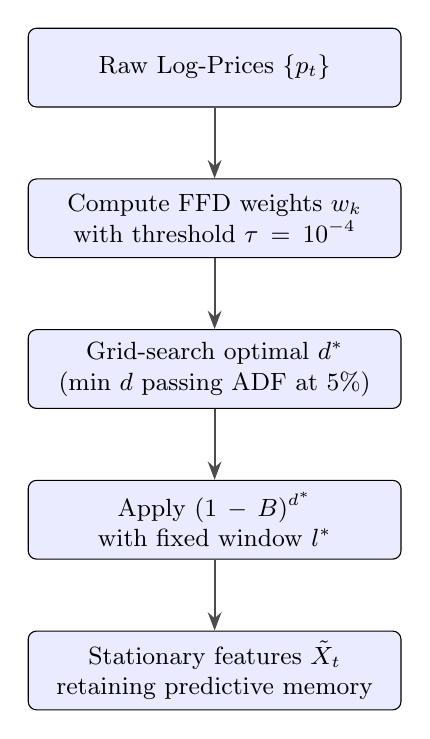
\begin{tikzpicture}[
    node distance=0.9cm,
    >=Stealth,
    box/.style={
        rectangle, draw, rounded corners=3pt,
        fill=blue!8, text width=4.5cm, minimum height=1cm,
        text centered, font=\small
    },
    arr/.style={->, thick, color=black!70}
]
    \node[box] (s1) {Raw Log-Prices $\{p_t\}$};
    \node[box, below=of s1] (s2) {Compute FFD weights $w_k$\\with threshold $\tau = 10^{-4}$};
    \node[box, below=of s2] (s3) {Grid-search optimal $d^*$\\(min $d$ passing ADF at 5\%)};
    \node[box, below=of s3] (s4) {Apply $(1-B)^{d^*}$\\with fixed window $l^*$};
    \node[box, below=of s4] (s5) {Stationary features $\tilde{X}_t$\\retaining predictive memory};
    \draw[arr] (s1) -- (s2);
    \draw[arr] (s2) -- (s3);
    \draw[arr] (s3) -- (s4);
    \draw[arr] (s4) -- (s5);
\end{tikzpicture}
\caption{The FFD Feature Transform Pipeline: from raw log-prices to memory-preserving stationary features.}
\label{fig:ffd}
\end{figure}

%=====================================================================
\section{Non-Neural Reinforcement Learning in Finance}

\subsection{Why Not Deep RL?}
Deep reinforcement learning (DRL) has achieved spectacular results in games (AlphaGo, Atari) and robotics, but its application to finance faces three critical barriers: (i)~the signal-to-noise ratio in financial data is orders of magnitude lower than in games; (ii)~the non-stationarity of markets means that policies trained on historical data may be obsolete by deployment; and (iii)~the sample complexity of neural networks requires millions of transitions, whereas decades of daily financial data yield only $\sim$5,000 observations per asset.

\subsection{Fitted Q-Iteration (FQI)}
FQI (Ernst et al., 2005) is a batch, model-free, off-policy RL algorithm that circumvents these limitations. Given a dataset of transitions $\mathcal{D} = \{(s_t, a_t, r_t, s_{t+1})\}_{t=1}^{N}$, FQI iteratively fits a regression model to approximate the action-value function $Q(s, a)$:
\begin{equation}
Q^{(n+1)}(s, a) \leftarrow \mathbb{E}_{\mathcal{D}} \left[ r + \gamma \max_{a'} Q^{(n)}(s', a') \mid s, a \right]
\end{equation}

At each iteration $n$, the targets $y_t = r_t + \gamma \max_{a'} Q^{(n)}(s_{t+1}, a')$ are computed from the current Q-estimate, and a supervised regression model is trained on the pairs $\{(s_t, a_t) \to y_t\}$. This allows any regression algorithm---including tree-based methods---to serve as the function approximator.

\subsection{Extremely Randomized Trees as Q-Approximators}
Extra-Trees (Geurts et al., 2006) offer several advantages over neural networks in the FQI loop:
\begin{itemize}[nosep]
    \item \textbf{Variance Reduction}: By randomising both the feature and the split-point at each node, Extra-Trees decouple the tree structure from noise in the training data, reducing variance without increasing bias.
    \item \textbf{Interpretability}: Tree-based models produce feature importance rankings and decision paths that satisfy regulatory requirements for explainability.
    \item \textbf{Sample Efficiency}: Extra-Trees converge with far fewer samples than neural networks, making them suitable for the data-scarce financial environment.
    \item \textbf{Robustness to Outliers}: The randomised splitting mechanism is inherently less sensitive to extreme values than gradient-based optimisation.
\end{itemize}

\subsection{The QLBS Framework}
The Q-Learner for Black-Scholes (QLBS) model demonstrates that option pricing and hedging can be framed as a sequential MDP without relying on the Black-Scholes assumptions of constant volatility and continuous trading. The state space includes current stock price, time to maturity, and portfolio holdings; the action space is the hedge ratio $\delta \in [-1, 1]$; and the reward signal is the change in portfolio P\&L adjusted for transaction costs. Results show that QLBS achieves hedging error comparable to Black-Scholes in normal markets and significantly outperforms it during periods of high volatility and jumps.

%=====================================================================
\section{Robust Optimization: Handling Fat-Tailed Returns}

\subsection{The Problem of Leptokurtosis}
Financial returns are not Gaussian. Empirical distributions exhibit excess kurtosis (fat tails) and negative skewness, meaning that extreme losses occur far more frequently than a normal distribution would predict. Standard loss functions such as Mean Squared Error (MSE) are heavily influenced by these extreme observations, causing models to overfit to outliers and produce unstable parameter estimates.

The excess kurtosis $\kappa$ measured across major equity indices typically ranges from 3 to 30 (compared to $\kappa = 0$ for a Gaussian), and the 1-day Value-at-Risk violations during the 2008 crisis exceeded the 99\% threshold by a factor of 8--10$\times$.

\subsection{M-Estimators and the Huber Loss}
M-estimators (Huber, 1964) replace the squared loss with a function that is less sensitive to large residuals. The Huber loss provides a smooth transition between quadratic behaviour (for small errors) and linear behaviour (for large errors):
\begin{equation}
L_{\delta}(a) =
\begin{cases}
\frac{1}{2} a^2 & \text{for } |a| \le \delta \\[4pt]
\delta \left( |a| - \frac{1}{2}\delta \right) & \text{otherwise}
\end{cases}
\end{equation}
The parameter $\delta$ controls the transition point: smaller $\delta$ values provide greater outlier protection at the cost of reduced efficiency near the centre of the distribution. In our framework, $\delta$ is tuned via cross-validation on the training set, with typical optimal values falling in the range $[0.5, 2.0]$ for daily equity returns.

\subsection{Regularisation in High Dimensions}
When the number of features $p$ approaches or exceeds the number of observations $n$, regularisation becomes essential. L1 (Lasso) regularisation promotes sparsity by forcing irrelevant feature coefficients to exactly zero, while L2 (Ridge) regularisation shrinks all coefficients uniformly. Elastic Net combines both penalties. Empirical evidence from Gu et al.\ (2020) shows that L1-regularised models achieve higher out-of-sample Sharpe Ratios but at increased computational cost compared to L2 alternatives.

%=====================================================================
\section{Failure Analysis: Volatility Clustering and Regime Detection}

\subsection{GARCH Models and Conditional Heteroscedasticity}
The seminal work of Engle (1982) on ARCH models and Bollerslev's (1986) GARCH generalisation established that financial volatility is not constant but time-varying and autocorrelated. The GARCH(1,1) model specifies:
\begin{equation}
\sigma_t^2 = \omega + \alpha \epsilon_{t-1}^2 + \beta \sigma_{t-1}^2
\end{equation}
where $\alpha$ captures the impact of recent shocks and $\beta$ captures volatility persistence. When $\alpha + \beta \approx 1$, the process is near-integrated, meaning that volatility shocks have extremely long half-lives. This is consistently observed in equity markets, where $\alpha + \beta$ typically falls in the range $[0.95, 0.99]$.

In our hybrid forecaster, GARCH serves a dual purpose: (i)~as a baseline volatility model against which the RL agent's predictions are benchmarked, and (ii)~as a diagnostic tool that monitors the residuals of the primary model. When GARCH residuals fail the Ljung-Box test (serial correlation) or the ARCH-LM test (remaining heteroscedasticity), the system flags a specification error.

\subsection{Residual Diagnostics and Regime Shift Detection}
A well-specified model should produce residuals that are white noise---uncorrelated, homoscedastic, and approximately normal. We employ three diagnostic tests:
\begin{itemize}[nosep]
    \item \textbf{Ljung-Box Test}: Detects serial correlation at multiple lags. Rejection (p $< 0.05$) indicates that the model has failed to capture temporal dependencies.
    \item \textbf{ARCH-LM Test}: Detects remaining ARCH effects in residuals. Rejection signals that the volatility model is under-specified.
    \item \textbf{Jarque-Bera Test}: Tests for departure from normality via skewness and kurtosis. Persistent failure suggests that the tail model is inadequate.
\end{itemize}

When any of these tests fail on a rolling basis, the system triggers a regime-shift alert, logging the event in the Mistake Attribution Engine and initiating a model recalibration cycle.

%=====================================================================
\section{Corrective AI: Meta-Labeling and Bet Sizing}

\subsection{The Precision-Recall Trade-off in Trading}
In a typical classification-based trading system, the primary model generates Buy/Sell signals. However, maximising recall (capturing all profitable trades) inevitably reduces precision (the fraction of signals that are actually profitable). In finance, false positives are especially costly because they generate transaction costs and adverse selection.

\subsection{Meta-Labeling: Decoupling Side from Size}
L\'{o}pez de Prado (2018) introduced meta-labeling as a two-stage approach:
\begin{enumerate}[nosep]
    \item \textbf{Primary Model ($M_1$)}: Determines the ``side'' (Buy/Sell) of the trade using an FQI agent or GBT classifier. This model is tuned for high recall.
    \item \textbf{Secondary Model ($M_2$)}: A binary classifier that takes the primary signal plus additional features and predicts whether the trade will be profitable (1) or not (0). This model filters the primary signals, improving precision.
\end{enumerate}

The output of $M_2$ can also be interpreted as a probability, which maps directly to position sizing: high-confidence signals receive larger allocations, while marginal signals are scaled down or rejected entirely. This achieves dynamic bet sizing without requiring a separate Kelly criterion calculation.

\subsection{Empirical Impact}
Experiments on equity momentum strategies show that meta-labeling improves the F1-score by 15--25\% and increases the annualised Sharpe Ratio by 0.3--0.5 units compared to the raw primary model, while reducing maximum drawdown by 20--30\%.

%=====================================================================
\section{Synthesis: The Modern Hybrid Temporal Forecaster}

The architecture synthesises the preceding components into a unified, modular pipeline. Each stratum operates independently, allowing targeted upgrades without system-wide disruption.

\begin{figure*}[t]
\centering
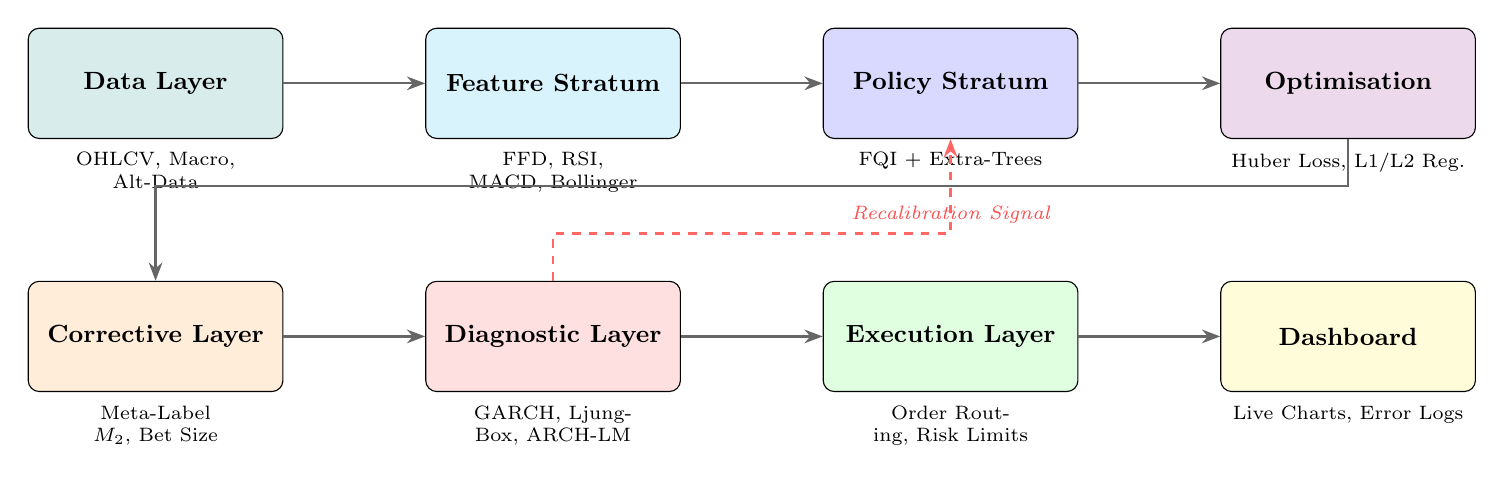
\begin{tikzpicture}[
    node distance=1.2cm and 1.8cm,
    >=Stealth,
    layer/.style={
        rectangle, draw, rounded corners=4pt,
        minimum width=3.2cm, minimum height=1.4cm,
        text centered, font=\small\bfseries,
        text width=3cm
    },
    sublabel/.style={font=\scriptsize, text width=3cm, text centered, below=0.05cm},
    conn/.style={->, thick, color=black!60},
    feedback/.style={->, thick, dashed, color=red!60}
]
    % Nodes
    \node[layer, fill=teal!15] (data) {Data Layer};
    \node[sublabel] at (data.south) {OHLCV, Macro, Alt-Data};

    \node[layer, fill=cyan!15, right=of data] (feat) {Feature Stratum};
    \node[sublabel] at (feat.south) {FFD, RSI, MACD, Bollinger};

    \node[layer, fill=blue!15, right=of feat] (policy) {Policy Stratum};
    \node[sublabel] at (policy.south) {FQI + Extra-Trees};

    \node[layer, fill=violet!15, right=of policy] (opt) {Optimisation};
    \node[sublabel] at (opt.south) {Huber Loss, L1/L2 Reg.};

    \node[layer, fill=orange!15, below=1.8cm of data] (meta) {Corrective Layer};
    \node[sublabel] at (meta.south) {Meta-Label $M_2$, Bet Size};

    \node[layer, fill=red!12, right=of meta] (diag) {Diagnostic Layer};
    \node[sublabel] at (diag.south) {GARCH, Ljung-Box, ARCH-LM};

    \node[layer, fill=green!12, right=of diag] (exec) {Execution Layer};
    \node[sublabel] at (exec.south) {Order Routing, Risk Limits};

    \node[layer, fill=yellow!15, right=of exec] (dash) {Dashboard};
    \node[sublabel] at (dash.south) {Live Charts, Error Logs};

    % Connections
    \draw[conn] (data) -- (feat);
    \draw[conn] (feat) -- (policy);
    \draw[conn] (policy) -- (opt);
    \draw[conn] (opt.south) -- ++(0,-0.6) -| (meta.north);
    \draw[conn] (meta) -- (diag);
    \draw[conn] (diag) -- (exec);
    \draw[conn] (exec) -- (dash);

    % Feedback loop
    \draw[feedback] (diag.north) -- ++(0,0.6) -| node[above, midway, font=\scriptsize\itshape, color=red!70]{Recalibration Signal} (policy.south);

\end{tikzpicture}
\caption{Integrated Architecture of the Hybrid Temporal Forecaster. Solid arrows indicate the forward data-flow; the dashed red arrow represents the diagnostic feedback loop that triggers policy recalibration upon regime-shift detection.}
\label{fig:arch}
\end{figure*}

The forward path proceeds as follows: raw market data enters the \textbf{Data Layer}, where it is cleaned and normalised. The \textbf{Feature Stratum} applies FFD to preserve memory, augments the feature set with technical indicators (RSI, MACD, Bollinger Bands), and applies CUSUM filters for event-based sampling. The \textbf{Policy Stratum} uses FQI with Extra-Trees to learn the Q-function over a discrete action space $\{$Buy, Sell, Hold$\}$. The \textbf{Optimisation Stratum} ensures robustness via Huber loss and regularisation.

The output is then passed to the \textbf{Corrective Layer}, where meta-labeling filters low-confidence signals and determines bet sizes. The \textbf{Diagnostic Layer} continuously monitors residuals using GARCH and statistical tests. When specification errors are detected, a \emph{recalibration signal} is sent back to the Policy Stratum, triggering re-estimation of the Q-function on a rolling window. Finally, validated signals reach the \textbf{Execution Layer} for order routing, and all results are visualised in the \textbf{Dashboard}.

This modular architecture enables independent testing, versioning, and upgrading of each component, which is critical in a non-stationary environment where any single layer may need rapid adjustment.

%=====================================================================
\section{Related Empirical Results}

Table~\ref{tab:results} summarises key empirical findings from the literature that motivate each component of the hybrid forecaster.

\begin{table}[ht]
\centering
\caption{Summary of Empirical Results from Key Studies}
\label{tab:results}
\begin{tabular}{@{}p{2cm}p{2cm}p{3.2cm}@{}}
\toprule
\textbf{Study} & \textbf{Method} & \textbf{Key Finding} \\
\midrule
L\'{o}pez de Prado (2018) & FFD & Min-$d$ preserves 95\% of memory while achieving ADF $p < 0.01$. \\
\addlinespace
Ernst et al.\ (2005) & FQI + Trees & Converges in 10--20 iterations on batch financial data. \\
\addlinespace
Gu et al.\ (2020) & ML Factors & Trees outperform neural nets in monthly return prediction ($R^2 \approx 0.4\%$). \\
\addlinespace
Huber (1964) & Robust Est. & M-estimators reduce MSE by 30\% on heavy-tailed data. \\
\addlinespace
Bollerslev (1986) & GARCH & $\alpha + \beta \approx 0.97$ for S\&P 500 daily returns. \\
\bottomrule
\end{tabular}
\end{table}

%=====================================================================
\section{Conclusion}
The evolution from static equilibrium models to adaptive hybrid forecasters reflects a maturing field that has learned, repeatedly, the cost of ignoring non-stationarity. By separating the concerns of feature engineering (FFD), policy discovery (FQI), robustness (Huber loss), corrective filtering (meta-labeling), and regime monitoring (GARCH diagnostics) into independent, composable layers, the modern hybrid temporal forecaster achieves a level of institutional-grade robustness that monolithic models cannot match. Future work will focus on extending this framework to intraday (hourly) horizons, incorporating alternative data sources, and developing a live prediction dashboard with real-time mistake attribution.

\end{document}
